% !TEX program = xelatex
\documentclass[paper=a4, titlepage, fontsize=11pt, parskip=full]{scrreprt}

% german names
\usepackage{ngerman}
% utf-8
\usepackage{polyglossia}
\setmainlanguage[spelling=new]{german}
\usepackage{fontspec}
\usepackage{pdfpages}

% In order to remove scr warning
\usepackage{scrhack}

%Needed to wrap text around images, used for personas
\usepackage{wrapfig}

%Used to avoid page breaks with each chapter
\usepackage{etoolbox}
\makeatletter
\patchcmd{\chapter}{\if@openright\cleardoublepage\else\clearpage\fi}{}{}{}
\makeatother

% colors
\usepackage{color}
\definecolor{grey}{rgb}{0.2,0.2,0.2}
\definecolor{orange}{rgb}{1,0.3,0}
\definecolor{turqoise}{rgb}{0,0.7,0.5}
\definecolor{OliveGreen}{rgb}{0.2,0.7,0.4}
\definecolor{Plum}{rgb}{0.52,0,0.7}

% Correctly break urls at hyphens
\usepackage[hyphens]{url}

% Special Link color (same as cite color)
\usepackage[colorlinks=true, citecolor=magenta, linkcolor=magenta, urlcolor=magenta] {hyperref}

%Black to save some costs
%\usepackage[colorlinks=true, citecolor=black, linkcolor=black, urlcolor=black] {hyperref}


% Use more than one optional parameter in a new commands
\usepackage{xargs}

% Adds Todos to output
\usepackage[colorinlistoftodos,prependcaption,textsize=tiny]{todonotes}
\newcommandx{\unsure}[2][1=]{\todo[linecolor=red,backgroundcolor=red!25,bordercolor=red,#1]{#2}}
\newcommandx{\change}[2][1=]{\todo[linecolor=blue,backgroundcolor=blue!25,bordercolor=blue,#1]{#2}}
\newcommandx{\info}[2][1=]{\todo[linecolor=OliveGreen,backgroundcolor=OliveGreen!25,bordercolor=OliveGreen,#1]{#2}}
\newcommandx{\improvement}[2][1=]{\todo[linecolor=Plum,backgroundcolor=Plum!25,bordercolor=Plum,#1]{#2}}
\newcommandx{\thiswillnotshow}[2][1=]{\todo[disable,#1]{#2}}

% To display figures exactly there where you want them to be
\usepackage[section]{placeins}

%Place subsections figures where you want them to be
\makeatletter
\AtBeginDocument{%
  \expandafter\renewcommand\expandafter\subsection\expandafter{%
    \expandafter\@fb@secFB\subsection
  }%
}
\makeatother

% code listings
\usepackage{listings}
\newcommand*\lstinputpath[1]{\lstset{inputpath=#1}}
\lstinputpath{Code}

\renewcommand{\lstlistingname}{Code}
\renewcommand{\lstlistlistingname}{Quellcodeverzeichnis}

\renewcommand*{\figureautorefname}{Ab\-bil\-dung}
\renewcommand*{\sectionautorefname}{Ab\-schnitt}
\renewcommand*{\chapterautorefname}{Ka\-pi\-tel}
\renewcommand*{\subsectionautorefname}{Ab\-schnitt}
\renewcommand*{\subsubsectionautorefname}{Ab\-schnitt}
\newcommand{\lstnumberautorefname}{Zeile}


\lstdefinelanguage{scala}{
  morekeywords={abstract,case,catch,class,def,%
    do,else,extends,false,final,finally,%
    for,if,implicit,import,match,mixin,%
    new,null,object,override,package,%
    private,protected,requires,return,sealed,%
    super,this,throw,trait,true,try,%
    type,val,var,while,with,yield},
  otherkeywords={=>,<-,<\%,<:,>:,\#,@},
  sensitive=true,
  morecomment=[l]{//},
  morecomment=[n]{/*}{*/},
  morestring=[b]",
  morestring=[b]',
  morestring=[b]"""
}

\lstdefinelanguage{buildSbt}{
  morekeywords={libraryDependencies},
  otherkeywords={+=, \%},
  sensitive=true,
  morecomment=[l]{//},
  morecomment=[n]{/*}{*/},
  morestring=[b]",
  morestring=[b]'
}

% Style languages
\lstdefinestyle{Code}{
	language=sql,
	basicstyle={\ttfamily \small},
	breaklines=true,
	commentstyle=\color{grey},
	keywordstyle=\color{orange},
	numbers=left,
	showspaces=false,
	captionpos=t,
	abovecaptionskip=12pt,
	stringstyle=\color{turqoise},
	xleftmargin=20pt
}
\lstdefinestyle{JSON}{
	string=[s]{"}{"},
	stringstyle=\color{blue},
	comment=[l]{:},
	commentstyle=\color{black},
	showspaces=false,
	captionpos=t,
	abovecaptionskip=12pt,
	xleftmargin=20pt
}
\lstdefinestyle{scala}{%
	basicstyle={\ttfamily \small},
	breaklines=true,
	commentstyle=\color{grey},
	keywordstyle=\color{orange},
	numbers=left,
	showspaces=false,
	stringstyle=\color{turqoise},
	xleftmargin=20pt
}

\lstdefinestyle{buildSbt}{%
	basicstyle={\ttfamily \small},
	breaklines=true,
	commentstyle=\color{grey},
	keywordstyle=\color{orange},
	numbers=none,
	showspaces=false,
  stringstyle=\color{turqoise}
}

\lstset{%
	language=bash,
	basicstyle={\ttfamily \small},
	breaklines=true,
	escapeinside={~}{~},
	postbreak=\mbox{\textcolor{red}{$\hookrightarrow$}\space},
	commentstyle=\color{grey},
	keywordstyle=\color{black},
  stringstyle=\color{black},
	otherkeywords={},
	numbers=none,
	showspaces=false,
	xleftmargin=\fboxsep,
  frame=lrb,
  xrightmargin=-\fboxsep,
  aboveskip=15pt,
  escapeinside={|}{|}
}

% This is necessary in order to avoid stupid latex errors, which are caused by importing gensymb package.
\usepackage{textcomp}

% Used for the degree symbol
\usepackage{gensymb}

% Place caption beneath listing
\usepackage[skip=12pt]{caption}

% Adding the source of a picture beneath it
\usepackage{subcaption}

%for images that are wrapped with text
\usepackage{wrapfig}
\usepackage{ragged2e}
\DeclareCaptionFormat{myformat}{#1#2\\#3}
\DeclareCaptionFont{white}{\color{white}}
\DeclareCaptionFormat{listing}{%
  \parbox{\textwidth}{\colorbox{darkgray}{\parbox{\textwidth}{#1#2#3}}\vskip -4pt}}
\captionsetup[lstlisting]{format=listing,labelfont=white,textfont=white}

% For adding the titelpage as a pdf
\usepackage{pdfpages}

% graphics
\usepackage{graphicx}
\graphicspath{{Images/}}

% BibTex lib - used for citation
%\usepackage{cite}

% Alternative to using common cite.

% Continuous footnote numbering (usually reset after chapter)
\usepackage{chngcntr}
\counterwithout{footnote}{chapter}

\usepackage[automark,headsepline,autooneside=false]{scrlayer-scrpage}
\clearpairofpagestyles{}
\ihead{\leftmark}
\chead{}
\ohead{\ifstr{\rightmark}{\leftmark}{}{\rightmark}}
%\ifoot{Bachelorthesis --- Tobias Kerst}
%\cfoot{}
\ofoot*{\pagemark}
\pagestyle{scrheadings}
\setkomafont{pageheadfoot}{\normalfont}

% Better layout size at footer and header
% footskip = is the dimension used as the baselineskip in the footer
\setlength\footskip{2cm}
\setlength\textheight{21.5cm}
%distance between the bottom of the text block and the top of the footer is
\setlength{\skip\footins}{1cm}
\setlength{\headsep}{1.5cm}
% Creates a bigger margin from page to header
%\usepackage[top=4cm]{geometry}
\setlength{\voffset}{0.8cm}

% Better footnote layout
\usepackage[bottom,hang]{footmisc}
\setlength{\footnotemargin}{1.2em}

\usepackage{lipsum}

\setkomafont{disposition}{\normalfont\bfseries}

% for verbatiminput
\usepackage{verbatim}

% Used for cross-referencing between different files
\usepackage{xr}

% German quotation marks
\let\oldquote'
\newif\ifquoteopen
\catcode`\'=\active
\makeatletter
% we have to redefine \pr@m@s to use an active '
\def\pr@m@s{%
  \ifx'\@let@token
    \expandafter\pr@@@s
  \else
    \ifx^\@let@token
      \expandafter\expandafter\expandafter\pr@@@t
    \else
      \egroup
    \fi
  \fi}
\protected\def'{%
  \ifmmode
    \expandafter\active@math@prime
  \else
    \expandafter\active@text@prime
  \fi}
\def\active@text@prime{%
   \@ifnextchar'{%
     \ifquoteopen
       \global\quoteopenfalse\grqq\expandafter\@gobble
     \else
       \global\quoteopentrue\glqq\expandafter\@gobble
     \fi
   }{%
     \ifquoteopen
       \global\quoteopenfalse\grq\xspace
     \else
       \global\quoteopentrue\glq
     \fi
   }%
}
\makeatother

% not yet used
%\input{src/cmd}

% Defines a macro \Autoref to allow multiple references to be passed to \autoref
\makeatletter
\newcommand\Autoref[1]{\@first@ref#1,@}
\def\@throw@dot#1.#2@{#1}% discard everything after the dot
\def\@set@refname#1{%    % set \@refname to autoefname+s using \getrefbykeydefault
    \edef\@tmp{\getrefbykeydefault{#1}{anchor}{}}%
    \def\@refname{\@nameuse{\expandafter\@throw@dot\@tmp.@autorefname}n}%
}
\def\@first@ref#1,#2{%
  \ifx#2@\autoref{#1}\let\@nextref\@gobble% only one ref, revert to normal \autoref
  \else%
    \@set@refname{#1}%  set \@refname to autoref name
    \@refname~\ref{#1}% add autoefname and first reference
    \let\@nextref\@next@ref% push processing to \@next@ref
  \fi%
  \@nextref#2%
}
\def\@next@ref#1,#2{%
   \ifx#2@ und~\ref{#1}\let\@nextref\@gobble% at end: print and+\ref and stop
   \else, \ref{#1}% print  ,+\ref and continue
   \fi%
   \@nextref#2%
}
\makeatother

% avoids schusterjungen and hurenkinder
\usepackage[all]{nowidow}
\clubpenalty10000
\widowpenalty10000
\displaywidowpenalty=10000


\begin{document}
\title{Telegram-Bot für Fakultätsnachrichten \\ - \\ Chatbot mit Rivescript}
\subtitle{Projektarbeit}
\author{%
	Tobias Kerst (62266) \\
  Anna-Lena Schwarzkopf (62265) \\
  Phillip Geis (63344) \\
  INFM
}
\date{Sommersemester 2018}
\publishers{
    \textbf{Professor:} Prof. Dr. rer. nat. Peter A. Henning
}
\maketitle

\clearpage

\pagenumbering{gobble}
\phantomsection\addcontentsline{toc}{chapter}{Inhaltsverzeichnis}
\begingroup
\hypersetup{linkcolor=black}
\tableofcontents
\endgroup

\clearpage


\pagenumbering{arabic}
\chapter{Einführung}

Nachdem der IWINewsBot im vergangenen Semester seine Grundfunktionalitäten erhalten hat, wurde in diesem Semester weiter an ihm gearbeitet. Diese Projektarbeit war fokussiert auf die Implementierung von Chatbot-Funktionalitäten mithilfe von Rivescript, sodass eine natürliche Interaktion mit dem Bot möglich wird. 

Neben dem Anbieten von bereits existierenden Funktionen, wie dem Mensaplan sollten auch neue Funktionen wie die Abfrage des Stundenplans möglich sein.
In dieser Dokumentation werden die neuen Funktionen vorgestellt und die Implementierung dieser beschrieben. Neben den Chatbot-Funktionen wurde auch weiter an der Robustheit des Bots gearbeitet und bestehende Funktionalitäten wurden verbessert und erweitert.
\chapter{Rivescript} \label{sec:rivescript}
Rivescript beschreibt sich selbst als einfache Skriptsprache, die Chatbots Intelligenz gibt.~\footnote{\url{https://www.rivescript.com/about}} Es ermöglicht in einem gewissen Rahmen eine Konversation des Benutzers mit dem Chatbot innerhalb eines Kontextes aufrecht zu erhalten. Eine weitere Funktion ist zum Beispiel das Merken von Variablen.

Bei dieser Projektarbeit werden solche erweiterten Funktionen nicht benötigt. Das Hauptszenario ist, dass der Benutzer dem Bot eine Frage stellt. Diese Frage wertet der Bot aus und liefert die entsprechenden Informationen zurück. Die Unterhaltung beschränkt sich also meistens auf eine Frage und eine Antwort.

\section{Vorstellung}
Rivescript wird einfach mithilfe eines Texteditors in eine \texttt{.rive}-Datei geschrieben, die von einem Interpreter ausgelesen und ausgewertet wird. Es werden im Bezug auf den Interpreter derzeit die Sprachen \texttt{Go}, \texttt{Java}, \texttt{JavaScript}, \texttt{Perl} und \texttt{Python} direkt von den Rivescript Entwicklern und \texttt{C\#} und \texttt{PHP} von Drittentwicklern unterstützt. Die erste unterstützte Sprache war Perl.

Rivescript funktioniert nach einem einfachen Trigger-Response-Prinzip. Die Eingabe des Benutzers wird ausgelesen und es wird in festgelegten Ausdrücken gesucht, ob sie mit einem Ausdruck übereinstimmt. Ist dies der Fall, antwortet der Bot mit der entsprechenden Antwort.
Ein einfaches Rivescript-Programm könnte also lauten:
\lstinputlisting[firstline=1, lastline=4, numbers=none, caption=Einfaches Rivescript-Programm, label=basicRive]{riveExamples.rive}

Das ''\textbf{+}''-Symbol stellt dabei die Eingabe des Users, das ''\textbf{-}''-Symbol die Ausgabe des Bots da. So können auf eine Eingabe verschiedene Ausgaben passen, bei denen dann zufällig ausgewählt wird, welche der Bot zurückgibt. Den Ausgaben kann aber auch eine gewisse Gewichtung gegeben werden, die dann eine feste Wahrscheinlichkeit der Antworten vorgibt.
\lstinputlisting[firstline=3, lastline=5, numbers=none, caption=Gewichtete Ausgaben in Rivescript, label=weight]{riveExamples.rive}

Rivescript bietet die Möglichkeit sprachliche Alternativen bekannt zu machen, sodass bei unterschiedlichen Schreibweisen trotzdem eine passende Eingabe gefunden werden kann.
Mit dem Schlüsselwort \emph{! sub} können so Abkürzungen bekannt gemacht werden.
\lstinputlisting[firstline=7, lastline=9, numbers=none, caption=Automatischer Austausch von sinngleichen Wörtern in Rivescript, label=subs]{riveExamples.rive}

Man möchte jedoch nicht nur auf komplett festgesetzte Sätze matchen, sondern auch auf ''vagere'' Aussagen. Dafür stellt Rivescript Wildcards bereit.
\lstinputlisting[firstline=11, lastline=12, numbers=none, caption=Wildcards in Rivescript, label=wildcards]{riveExamples.rive}

Das ''\textbf{*}''-Symbol steht für eine beliebige Anzahl von Wörtern und Zahlen. Dieses kann in der Antwort berücksichtigt werden und damit zum Beispiel, wie hier gezeigt,  als Aufrufparameter einer Methode benutzt werden.
Weitere Wildcards sind das ''\textbf{\_}''- und ''\textbf{\#}''-Symbol. Das ''\textbf{\_}''-Symbol fordert ein Wort ohne Zahlen und Leerzeichen, das ''\textbf{\#}''-Symbol eine Zahl.
Weiterhin gibt Rivescript die Möglichkeiten Arrays anzulegen, die in der Eingabe des Benutzers enthalten sein können, wie zum Beispiel Farben.
\lstinputlisting[firstline=15, lastline=18, numbers=none, caption=Arrays in Rivescript, label=array]{riveExamples.rive}

In Rivescript erhalten die Klammertypen verschiedene Aufgaben. Bei runden Klammern ist es möglich für die Ausgabe des Bots den Inhalt der Klammern als Parameter zu benutzen oder es wie im zuvor genannten Beispiel direkt auszugeben.

Durch die Worte in eckigen Klammern erhält der Eingabesatz eine bessere Struktur und die Wahrscheinlichkeit eine Übereinstimmung zu finden steigt, aber sie sind nicht als mögliche \texttt{<star>}-Parameter nutzbar. Sie sind optional.

Um mehrere Formulierungen in einem Satz abzudecken, ist es möglich Alternativen durch das Oder-Symbol aneinander zu hängen.
\lstinputlisting[firstline=21, lastline=22, numbers=none, caption=Mehrere Formulierungen durch Alternativen in einem Ausdruck, label=alternatives]{riveExamples.rive}

So sind die Formulierungen ''Wie sieht mein Stundenplan aus?'' und ''Was ist mein Stundenplan?'' beide in einem Fall abgedeckt. Hier gilt ebenfalls, dass der Inhalt von runden Klammern als Match verfügbar gemacht werden kann, eckige Klammern wären wieder nur optional. \\
Zu erwähnen gibt es noch, dass Rivescript-Satzzeichen in den erwarteten Eingaben des Users automatisch wegoptimiert. Es ist also lediglich notwendig grammatikalisch korrekte Sätze für die Ausgabe des Bots zu schreiben.

\section{Einbindung und Implementierung}
Die Einbindung in das bestehende Projekt war sehr einfach, da es für Rivescript bereits eine Java-Bibliothek gibt, die dem Projekt hinzugefügt werden kann. Die \texttt{build.sbt}-Datei muss hierbei um die folgende Zeile erweitert werden:
\lstinputlisting[language=buildSbt, style=buildSbt, numbers=none, caption=Auszug der build.sbt, label=buildSbt]{build.sbt}

\subsection{Reagieren auf Freitext}
Da der Bot bis zu diesem Zeitpunkt lediglich auf Commands reagiert hat, was durch die \texttt{onCommand}-Methoden umgesetzt wurde, musste der Bot zusätzlich auf normale Texteingaben reagieren, also auf Textnachrichten, die nicht mit einem Slash beginnen. Das \texttt{Telegrambot4s}-Framework bietet hierfür keine spezielle Methode, aber man kann auf allgemeinen Input reagieren.
Es wurde hierfür also eine neue Klasse erstellt, die zu den Commands gehört und auf Chat-Nachrichten reagiert. 
\lstinputlisting[language=scala, style=scala, caption=Abfangen der Freitextnachrichten in Chat.scala, label=chatScala1, firstline=1, lastline=15]{Chat.scala}

Wie man in \Autoref{line:inputSlash} erkennt, wird auf jede beliebige Nachricht reagiert und geprüft, ob die Nachricht mit einem Slash beginnt. Beginnt die Eingabe mit einem Slash, soll nicht weiter gearbeitet werden, da es hierfür optimierte Klassen und Methoden gibt. Beginnt die Eingabe jedoch nicht mit einem Slash, so handelt es sich also um Freitext. An dieser Stelle wird nun Rivescript eingesetzt um die Eingabe zu interpretieren.

\subsection{Rivescript-Chatbot}
Rivescript stellt eine eigene Klasse zur Verfügung, die genutzt werden kann um den Chatbot zu konfigurieren. Hierbei kann nicht nur eingestellt werden, welche \texttt{.rive}-Dateien der Bot nutzen soll, sondern es können auch Dinge wie \texttt{UTF-8}-Support eingestellt werden. Für den korrekten Umgang mit Umlauten in der deutschen Sprache ist dies eine Voraussetzung für den IWINewsBot.

Die einfachste Möglichkeit zum Setzen der Attribute wären Aufrufen von \texttt{Setter}-Methoden auf der von Rivescript bereitgestellten Rivescript-Klasse, um den Code aber modularer und verständlicher  zu machen, wurde eine eigene Klasse erstellt, die von Rivescript erbt und intern alle nötigen Einstellungen trifft. \newpage
\lstinputlisting[language=scala, style=scala, caption=Initialisierung von Rivescript und seiner Routinen, label=initRive]{ChatBot.scala}

Neben dem Setzen von \texttt{UTF-8} ist vor allem das Bekanntmachen der \texttt{.rive}-Dateien ein Bestandteil dieser Klasse und außerdem das Setzen von Routinen. Diese Routinen werden aus den \texttt{.rive}-Dateien aufgerufen und werden benötigt um programmatische Aufrufe zu tätigen, also Funktionen umzusetzen, die mit Rivescript alleine nicht möglich sind. Dies wird im Kapitel Implementierte Funktionen genauer betrachtet. \\
Der voll konfigurierte Chatbot kann nun genutzt werden, um Freitextnachrichten zu lesen, indem er als Singleton eingebunden wird und die Eingabe bekommt. Als Antwort erhält man entsprechend einen String. Wie dies konkret implementiert ist, wird im folgenden gezeigt:
\lstinputlisting[language=scala, style=scala, caption=Abfangen der Freitextnachrichten in Chat.scala, label=chatScala2, firstline=17, lastline=37]{Chat.scala}

Da der IWINewsBot als \texttt{.jar} gebaut wird und die Rivescript Dateien ein Teil des Programms sind, müssen diese auch in das \texttt{.jar} gepackt werden. Dies geschieht am einfachsten, indem die \texttt{.rive}-Dateien im \texttt{resources/}-Ordner abgelegt werden. \\
Das Laden hat sich als nicht trivial herausgestellt, es war nicht möglich die Dateien einfach als \texttt{File}-Objekte zu lesen, lediglich das Lesen als InputStream war möglich, was jedoch durch Rivescript möglich ist.
\chapter{Implementierung}
Nachdem nun die erwarteten Funktionen festgelegt sind, soll in diesem Kapitel die genauere Implementierung vorgestellt werden. Hierbei wird auch auf eine mögliche Erweiterbarkeit des Bots eingegangen.

Der Source Code des Bots ist auf Github über die Adresse \url{https://github.com/TobsCore/IWINewsBot} zu finden. Von dort aus kann der Code über den folgenden Befehl geladen werden.

\begin{lstlisting}
git clone https://github.com/TobsCore/IWINewsBot
\end{lstlisting}

In dem geladenen Ordner \texttt{IWINewsBot} befinden sich dabei die folgenden drei Ordner: \texttt{src}, \texttt{project} und \texttt{Documentation}. In \texttt{src/} sind die Dateien für den Bot enthalten, in \texttt{project/} befinden sich Informationen zu dem SBT-Projekt und in \texttt{Documentation} sind die Quelldateien für diese Dokumentation enthalten.

Damit der Bot korrekt starten kann, ist ein Token notwendig, hierzu legt man im Root-Ordner die Datei \texttt{bot.token} an und speichert in dieser Datei das vom BotFather generierte Token. Der Bot wird diese Datei dann nutzen, um sich zu verifizieren. Aus Sicherheitsgründen ist das Token nicht im Repository gespeichert.

\section{Scala und das Scala Build Tool}
Es wurde entschieden, den Bot in Scala zu programmieren, da dies eine interessante Programmiersprache ist, mit der man als Studierender nicht viele Berührungspunkte hat. Scala bietet durch die Objektorientierung vertraute Konzepte, jedoch sind viele Konzepte der funktionalen Programmierung in der Sprache vorhanden.

Um das Projekt zuverlässig bauen zu können und Abhängigkeiten zu verwalten, wird das Scala-Build-Tool (kurz \emph{SBT}) eingesetzt. Dieses Build-Tool gilt als Standard-Build-Tool für Scala Projekte. Um das Projekt besser kennen lernen zu können, soll an dieser Stelle die \texttt{build.sbt} des Projekts gezeigt werden, anhand derer SBT vorgestellt werden soll.

\lstinputlisting[language=scala, style=scala, caption=Übersicht der build.sbt]{build.sbt}

Am Anfang der Datei werden Informationen zu dem Projekt festgelegt, wie der Name und die Version. Außerdem kann an dieser Stelle die Scala-Version festgelegt werden.

Im Anschluss werden die Scala-Abhängigkeiten verwaltet. Wie man feststellt, setzt der Telegram-Bot Bibliotheken wie \emph{Scala Test}, \emph{Telegrambot4s} und die Logging-Engine \emph{Logback} ein. Diese Abhängigkeiten werden über den \texttt{+=} an \texttt{libraryDependencies} angehängt.

Außerdem kann festgelegt werden, in welcher Datei sich die Main-Methode befindet, also die Methode, mit der das Programm gestartet werden soll. Wie man an der \texttt{build.sbt} erkennt, befindet sich diese in der Klasse \texttt{IWINewsBot} und ist im Package \texttt{hska\allowbreak.iwi\allowbreak.telegramBot}.

Außerdem wurden noch ein paar Regeln festgelegt, die die Benutzung vereinfachen. Diese sind am Ende der Datei definiert.

\subsection{Kompilieren und Fat-Jar Generierung}
Um SBT nutzen zu können, muss dies installiert sein. Interessant ist, dass Scala nicht auf dem Computer installiert sein muss, es kann auch nachträglich von SBT bezogen und installiert werden. Um das Projekt zu kompilieren, wird im Terminal in den Projektorder navigiert. Folgender Befehl lässt sich dann ausführen:

\begin{lstlisting}[language=bash]
> sbt
\end{lstlisting}

Dadurch startet sich ein SBT-Server. Über diesen Server kann dann das Projekt einfach kompiliert und gestartet werden.

\begin{lstlisting}[language=bash]
sbt:IWINewsBot> compile
\end{lstlisting}

\begin{lstlisting}[language=bash]
sbt:IWINewsBot> run
\end{lstlisting}

Da einige Klassen auch durch Unit-Tests getestet werden, kann dies auch direkt über den SBT-Server gestartet werden (mittels \texttt{test}). Der SBT-Server kann über \texttt{exit} beendet werden. Die Nutzung des Servers ist dahingehend sinnvoll, dass viele Dateien gecachet werden können und das Projekt nicht jedes Mal neu geladen werden muss. Natürlich ist es auch möglich, das Projekt zu kompilieren, ohne den SBT-Server zu starten. Man kann aus der Kommandozeile auch folgendes eingeben:

\begin{lstlisting}[language=bash]
> sbt compile
\end{lstlisting}

Um das Programm dann jedoch auf einen Server zu spielen und dort zu starten, ist es sinnvoll, eine ausführbare Datei zu haben. Scala erzeugt JVM-Code, also gilt es eine \texttt{JAR}-Datei zu generieren. Um dieses JAR auf beliebigen Rechnern lauffähig zu machen, also auch auf Computern und Servern, die neben der JVM kein Scala installiert haben und zugleich auch alle Abhängigkeiten dazu zu packen, ist die Generierung eines sogenannten \emph{Fat-JAR}s notwendig.

Über das \emph{Assembly}-Plugin kann man genau dies umsetzen. Wenn man SBT gestartet hat, reicht die Ausführung des folgenden Befehls:

\begin{lstlisting}[language=bash]
> sbt assembly
\end{lstlisting}

Hierdurch wird das Programm \texttt{IWINewsBot\allowbreak-assembly\allowbreak-0.4\allowbreak.jar} in dem Ordner \texttt{target\allowbreak/scala-2.12/} generiert, wobei 0.4 für die (in der \texttt{build.sbt} eingestellten) Version steht. Navigiert man in diesen Ordner, kann das Programm dann durch Ausführung des Befehls \texttt{java -jar IWINewsBot-assembly-0.4.jar} der Bot gestartet werden.

\textbf{Wichtig:} Damit der Bot starten kann, ist es absolut notwendig, dass in dem selben Ordner die \texttt{bot.token}-Datei mit dem validen Token für den Bot liegt. Man müsste also die \texttt{bot.token}-Datei in den Ordner \texttt{./target/scala-2.12/} kopieren, damit man die JAR-Datei erfolgreich ausführen kann.

\subsection{Scalafmt}
Um einen einheitlichen Code zu schreiben, wird das Scalafmt\footnote{Siehe \url{http://scalameta.org/scalafmt/}}-Tool benutzt. Hierbei kann eine Konfiguration benutzt werden, um eigene Regeln festzulegen, ansonsten werden Standard-Regeln zu Formatierung des Codes eingesetzt. Die eigenen Regeln befinden sich in der Datei \texttt{.scalafmt.conf}. Für dieses Projekt wird das \emph{neo-sbt-scalafmt}-Plugin\footnote{Weitere Informationen zu dem Projekt findet man unter \url{https://github.com/lucidsoftware/neo-sbt-scalafmt}} eingesetzt.

Sollte der Bot mit einer IDE weiterentwickelt werden, so empfiehlt es sich ein Plugin zur automatischen Formatierung mit Scalafmt einzusetzen\footnote{Für die bisherige Entwicklung wurde IntelliJ eingesetzt, hierfür kann das Scalafmt Plugin von Olafur Pall Geirsson eingesetzt werden: \url{https://github.com/scalameta/scalafmt}}. Alternativ kann das Programm über die Kommandozeile in der SBT Shell (also über den SBT Server) ausgeführt werden:

\begin{lstlisting}
sbt:IWINewsBot> scalafmt
\end{lstlisting}

\section{Bot starten}
Im Folgenden wird erklärt, welche Schritte notwendig sind, damit der Bot gestartet werden kann.

Scala setzt auf die JVM als Laufzeitumgebung, weswegen es wichtig ist, dass ein JDK installiert ist, da die Software nicht nur lauffähig sein soll, sondern auch gebaut und gebündelt werden soll.

Um den Bot starten zu können, muss ein Bot bei Telegram über den BotFather erstellt werden. Hier erhält man dann im Anschluss das Token. Nun erstellt man im Hauptprojektordner eine neue Datei \texttt{bot.token} in der man das Token ohne nachfolgende Leerzeichen speichert.

Damit der Bot ohne Fehler starten kann, muss eine Rudis-Instanz, auf dem Port 6379, gestartet werden, was der Standardport für Redis ist. Bei Redis handelt es sich um eine sehr einfach gehaltene In-Memory Datenbank mit Persistenzmöglichkeit. Der Redis-Server wird über den Befehl

\begin{lstlisting}
> redis-server
\end{lstlisting}

gestartet.

Über den bereits besprochenen Befehl \texttt{sbt run} kann der Bot dann gestartet werden.

\section{Projektstruktur}
Das eigentliche Projekt befindet sich unter \texttt{src/}, wobei unter Projektcode (in dem Unterordner \texttt{main/}) und Testcode (in dem Unterordner \texttt{test/}) unterschieden wird. Wie auch bei Java werden in Scala Packages genutzt um Namespaces nachzubilden. Somit ist es möglich, Klassen mit gleichen Namen in einem Projekt zu nutzen. Für den Telegram-Bot wurde das Package \texttt{hska.iwi.telegramBot} gewählt. In diesem Package liegen direkt die Main-Klasse \texttt{IWINewsBot}, welche den Bot startet (siehe~\autoref{sec:Programmstart}).

\subsection{Kommandos}
Der Bot kommuniziert auf zwei Arten mit dem Nutzer. Zum einen kann der Nutzer den Bot über bestimmte Befehle direkt ansprechen, worauf dieser dann antwortet. Zum anderen verschickt der Bot automatisch Nachrichten an alle Subscriber, falls es neue Nachrichten gibt.

Für den ersten Fall gibt es die Klassen in dem Paket \texttt{hska\allowbreak.iwi\allowbreak.telegramBot\allowbreak.commands}, bei denen definiert wird, wie reagiert wird, wenn ein bestimmter Befehl an den Bot geschickt wird, wobei Befehle mit ein Slash beginnen müssen. Hierbei kann es sich um öffentliche Befehle handeln, also Befehle, die dem BotFather mitgeteilt werden, damit dieser die Befehle vorschlagen kann, es ist aber auch möglich, auf Befehle zu reagieren, die dem BotFather nicht bekannt gemacht wurden. Dies wurde vor allem während der Entwicklung genutzt, um bestimmte Funktionalitäten zu nutzen, die noch nicht ganz fertig waren, beispielsweise dem Setzen von Einstellungen, als die Inline-Buttons für diese Funktion noch nicht fertig implementiert waren.

Neben den Commands wird im Hintergrund der Fakultätsserver regelmäßig nach neuen Nachrichten abgefragt. Hierfür existiert die Klasse \texttt{BackgroundFeedSync}, die einen Actor\footnote{Actors sind eine moderne Abstraktionsschicht für nebenläufiges Verhalten, für mehr Informationen siehe: \url{http://danielwestheide.com/blog/2013/02/27/the-neophytes-guide-to-scala-part-14-the-actor-approach-to-concurrency.html}} startet, der im Hintergrund die Fakultätsserver abfragt, auf die Datenbank zugreift und im Falle einer neuen Nachricht die jeweiligen Subscriber benachrichtigt.

Die Ergebnisse der REST-Abfragen sind als JSON kodiert. Zur Deserialisierung werden Case-Klassen eingesetzt, die mithilfe von der \emph{JSON4S}- und \emph{Jackson}-Bibliothek gefüllt werden. Diese Case-Klassen befinden sich in verschiedenen Unterpackages, beispielsweise \texttt{mensa}, \texttt{news} oder \texttt{rooms}.

Zuletzt gibt es das Unterpackage \texttt{service} in der allerlei Helferklassen zusammengefasst werden. Neben der Auslagerung der einzelnen Web-Adressen der Fakultät wird dort die Datenbankanbindung und Wrapper für die HTTP-Requests gespeichert.

\subsection{Main Klasse}\label{sec:Programmstart}
Betrachtet man die Datei \texttt{IWINewsBot.scala}, so sieht man dort einmal die Klassendefinition von \texttt{IWINewsBot}, am Ende der Datei wird zudem aber auch ein \emph{object} mit dem Namen \texttt{IWINewsBot} erstellt, welches von \texttt{App} erbt. Bei diesem \emph{object} handelt es sich um die Main Klasse, also jene Klasse, die beim Aufruf des Programms gestartet wird. Alles im Rumpf des IWINewsBot-Objekts wird dabei ausgeführt. Wie man darin erkennen kann, wird einen Klasseninstanz von \texttt{IWINewsBot} erstellt und gestartet.

Die \texttt{IWINewsBot}-Klasse erbt von ganz vielen Klassen. Bei Scala wird die Mehrfachvererbung unterstützt, wobei die typischen Konflikte vermieden werden, indem es eine \emph{Hauptklasse} gibt, von der die primären Methoden stammen. Diese wird durch \emph{extends} hinzugefügt, alle anderen über \emph{with}. Die Bibliothek \emph{Telegrambot4s} basiert auf dem Cake-Pattern\footnote{Wie \emph{Telegrambot4s} das Cake Pattern umsetzt, wird auf \url{https://github.com/mukel/telegrambot4s/wiki/Design} beschrieben}, sodass verschiedene Funktionen über Vererbung einfügt werden, als Komposition.

Wie auf die einzelnen Befehle eines Users reagiert werden soll, ist in den Klassen aus dem Package \texttt{commands} definiert. Diese Funktion wird auch über Vererbung in den Bot eingefügt. Um die Funktionen besser zu kapseln wurden diese in verschiedene Klassen unterteilt, konkret in die Folgenden:

\begin{description}
  \item[Subscription] Generelle Abonnement-Befehle (\texttt{/start} und \texttt{/stop})
  \item[Mensa] \texttt{/mensa}- und \texttt{/settings}-Befehle
  \item[Lecturers] \texttt{/profs}-Befehl
  \item[AboSettings] \texttt{/abo}-Befehl
  \item[About] Informationen zum Bot, \texttt[/about]-Befehl
  \item[Admin] Admin-Funktionen, die von normalen Nutzern des Bots nicht ausgeführt werden können.
\end{description}

Sollte man eine weiter Klasse hinzufügen wollen, die auf bestimmte Befehle reagiert, so muss diese auch über das Cake-Pattern der Hauptklasse bekannt gemacht werden, also über \texttt{with Klassenname} hinzugefügt werden.

Damit ist erklärt, wie der Telegram-Bot auf Kommandos reagiert. Das Überprüfen auf neue Nachrichten soll, wie bereits beschrieben, im Hintergrund passieren. Die Klasse \texttt{BackgroundFeedSync} kümmert sich darum und wird deswegen auch in der Hauptklasse gestartet.

Zu guter Letzt muss das Bot-Token vom IWINewsBot geladen werden, weil es für die  Authentifizierung genutzt wird. Das Framework \emph{Telegrambot4s} regelt dies automatisch ab, es muss lediglich das Token in dem Value \texttt{token} gespeichert werden. Da das Token geheim bleiben muss, wird es aus der Datei \texttt{bot.token} gelesen.

\section{Kommandos}
Bevor auf die einzelnen Kommandos eingegangen wird und wie diese implementiert wurden, soll die generelle Konzeption der Kommando-Klasse eingegangen werden. Aus Übersichtlichkeitsgründen sollten diese Klassen im \texttt{commands}-Package abgelegt werden und als Trait implementiert werden, damit diese für das Cake Pattern genutzt werden können. Bei Traits handelt es sich um Interfaces mit konkreter Implementierung, damit wird die Mehrfachvererbung auf der JVM ermöglicht.

Der Aufbau soll anhand des erfunden \emph{Help}-Kommandos erklärt werden. Der Nutzer soll durch das Abschicken eines \texttt{/help}-Befehls einen Hilfetext angezeigt bekommen.

Das Trait \texttt{Help} würde dann wie folgt definiert:

\begin{lstlisting}[language=scala,style=scala,caption=Grundstruktur eines eigenen Kommandos]
trait Help extends Commands {
  _: TelegramBot =>

}
\end{lstlisting}

Um auf Befehle zu reagieren, wird die \texttt{onCommand} Methode genutzt. In unserem Beispiel, bei dem der User \texttt{/help} absendet, würde das dann wie folgt aussehen:

\begin{lstlisting}[language=scala, style=scala, caption=Reaktion auf den help-Befehl]
trait Help extends Commands {
  _: TelegramBot =>

  onCommand("/help") { implicit msg =>
   val helpMessage = "Über die reply() Methode wird eine Antwort verschickt."
   reply(helpMessage)
 }
}
\end{lstlisting}

Zu guter Letzt neben dem Absenden des Hilfetexts das Ereignis geloggt werden. Hierzu soll auf das Userobjekt zugegriffen werden, der den Befehl an den Bot geschickt hat. Hier bietet das Framework die nützliche \texttt{using}-Funktion.

\begin{lstlisting}[language=scala, style=scala, caption=Zugriff auf das User Objekt]
onCommand("/help") { implicit msg =>
    using(_.from) { user =>
      val userID = UserID(user.id)
      logger.info(s"User ${userID} requested help.")
      // Weitere Funktionen können hier folgen
    }
}
\end{lstlisting}

\subsection{Start- und Stop-Befehle}\label{sec:StartStopCommands}
Wenn man den Bot initial aufruft, wird die Unterhaltung über den Befehl \texttt{/start} gestartet. Diese Methode wird ausführlicher beschrieben, da an dieser Stelle auch die Persistenzschicht beschrieben wird.

\begin{lstlisting}[language=scala, style=scala, caption=Reagieren auf Start-Befehl]
onCommand("/start") { implicit msg =>
  using(_.from) { user =>
    {
      val userID = UserID(user.id)
      try {
        if (redis.addUser(userID)) {
          reply(
            """Du erhältst ab jetzt alle Nachrichten des schwarzen Bretts und der Fakultät IWI an der HSKA.
            |Um Deine Einstellungen anzupassen, wähle /abo aus.""".stripMargin)
          logger.info(s"${user.firstName} ${user.lastName.getOrElse("")} added to subscriptions.")
          logger.debug(s"$user is stored in Database")

          // Set configuration. Everything is set to true, since the user subscribes to all
          // subjects by default.
          redis.setUserConfig(userID, Map(INFB -> true, MKIB -> true, INFM -> true))
        } else {
          reply("Du erhälst bereits Nachrichten.")
        }

        // Update the user data
        redis.setUserData(userID, user)
        redis.setFacultyConfigForUser(userID, configValue = true)
      } catch {
        case rte: RuntimeException =>
          logger.error("Cannot connect to redis server")
          logger.debug(rte.getMessage)
      }
    }
  }
}
\end{lstlisting}

Interessant an dieser Stelle ist die Zeile 6, in der die UserID der Redis-Datenbank übergeben wird. Existiert der User bereits, so wird er entsprechend darüber informiert (dies kann auftreten, wenn er mehr als 1x den \texttt{/start}-Befehl abschickt). Ist der User noch nicht registriert, so wird automatisch eine initiale Konfiguration gespeichert (Zeile 15). Für diese beiden Teile soll der entsprechende Code gezeigt werden:

\begin{lstlisting}[language=scala, style=scala, caption=Hinzufügen eines Users zur Datenbank]
override def addUser(userID: UserID): Boolean = {
  redis.sadd("users", userID.id).getOrElse(0l).toInt == 1
}
\end{lstlisting}

Redis wird also über die selben Befehle aufgerufen, die auch in der offiziellen Dokumentation aufgeführt werden\footnote{Offizielle Redis Dokumentation: \url{https://redis.io/commands}}.

Über \texttt{sadd()} werden die UserIDs einem Set hinzugefügt. Somit dürfen UserIDs auch nur einmal in diesem Set auftauchen, weswegen die \texttt{sadd()}-Methode 1 zurück gibt, wenn eine UserID hinzugefügt werden kann und 0, wenn die UserID nicht hinzugefügt wird (da diese UserID bereits existiert).

Der Code für das Speichern der Konfiguration sieht wie folgt aus:

\begin{lstlisting}[language=scala, style=scala, caption=Setzen der Userkonfiguration]
override def setUserConfig(userID: UserID, userConfig: Map[Course, Boolean]): Boolean = {
  redis.hmset(s"config:${userID.id}", userConfig)
}
\end{lstlisting}

Die Konfiguration wird als HashSet gespeichert, wobei der Schlüssel des HashSets die UserID mit einem vorangestellten \textit{config:}. Startet ein User mit der ID \texttt{1234567} den Bot, so wird seine Konfiguration also unter \texttt{config:1234567} abgespeichert und kann über \texttt{hmgetall()} abgerufen werden.

\begin{lstlisting}[language=scala, style=scala, caption=Abrufen der Userkonfiguration]
override def getConfigFor(userID: UserID): Option[Map[Course, Boolean]] = {
  redis.hgetall1[Course, Boolean](s"config:${userID.id}")
}
\end{lstlisting}

Wenn ein User keine weiteren Nachrichten mehr erhalten möchte, so kann er durch den \texttt{/stop}-Befehl sein Abonnement beenden, dabei wird dann seine UserID aus dem Set aller UserIDs entfernt und auch die Konfiguration wird gelöscht.

\subsection{Der Profs-Befehl}
Der Profs-Befehl gibt eine Liste aller Professoren als anklickbare Inline-Buttons aus. Wird einer dieser Button angeklickt, so werden Informationen zu dem entsprechenden Professor angezeigt. In diesem Teil der Dokumentation wird der Fokus auf diese Inline-Buttons gelegt, aber auch wie die Requests an den Server gestellt werden. Auf Redis soll nicht weiter im Detail eingegangen werden, da die Befehle alle dem offiziellen Muster folgen.

\begin{lstlisting}[language=scala, style=scala, caption=Reaktion auf das /profs Kommando, label={code:profsCommand}]
var lecturers: Option[Seq[Lecturer]] = None

onCommand("/profs") { implicit msg =>
  logger.debug(s"${msg.from.getOrElse("")} requested data about lecturers")
  val content = HTTPGet.get(FeedURL.lecturer)
  if (content.isDefined) {
    //parses the json entries and stores them in a lecturers object
    lecturers = Some(JsonMethods.parse(content.get).extract[Seq[Lecturer]].sortBy(_.lastname))
    //reply(RoomFormatter.format(lecturers), parseMode = Some(ParseMode.HTML))

    logger.info(s"Received ${lecturers.get.size} Lecturers.")

    reply("Wähle einen Professor aus, zu dem Du genauere Informationen erhalten möchtest.",
          replyMarkup = Some(createInlineKeyboardMarkup(lecturers.get)))
  }
}
\end{lstlisting}

Mit dem Befehl \texttt{/profs} wird der Fakultätsserver nach Informationen zu den Professoren gefragt. Dieser Antwortet mit einem JSON, das in dem Value \texttt{content} gespeichert wird. Das JSON wird dann über \texttt{JsonMethods.parse} geparset und in \texttt{lecturers} gespeichert, einer Liste von Professoren. Der relevante Teil bei dieser Methode befindet sich jedoch am Ende, hier wird in die Antwort zusätzlich das \texttt{replyMarkup} gesetzt, indem die \texttt{createInlineKeyboardMarkup}-Methode angerufen wird.

\begin{lstlisting}[language=scala, style=scala, caption=Erstellen der Professor-Button]
def createInlineKeyboardMarkup(lecturersSet: Seq[Lecturer]): InlineKeyboardMarkup = {
  val buttonSeq =
    lecturersSet
      .map(lec => InlineKeyboardButton.callbackData(lec.lastname, tagLecturer(lec.id.toString)))

  InlineKeyboardMarkup.singleColumn(buttonSeq)
}
\end{lstlisting}

Die Telegram API bietet verschiedene Arten der Darstellung von InlineButtons an, in dem Profs-Beispiel sollen mehrere Buttons untereinander aufgelistet werden. Dies wird über die Factory-Methode \texttt{InlineKeyboardMarkup.singleColumn} ermöglicht. Für jeden Professor soll ein eigener Button erstellt werden, welche dann als Liste in \texttt{buttonSeq} landen.

Um auf das Anklicken der Buttons zu reagieren, werden diese noch mit einem Tag versehen, hierzu wird die \texttt{prefixTag}-Funktion des Telegrambot4s-Framework genutzt.

\begin{lstlisting}[language=scala, style=scala, caption=Benutzung von Tags zur Identifikation von Callback-Methoden]
def tagLecturer: String => String = prefixTag("Lecturer")
\end{lstlisting}

Diese Tags werden dann zur Identifikation der entsprechenden Callback-Methode genutzt, also jener Methode, die beim Anklicken eines Buttons aufgerufen wird.

\begin{lstlisting}[language=scala, style=scala, caption=Callback-Funktionalität bei Inline-Buttons, label=code:InlineCallback]
onCallbackWithTag("Lecturer") { implicit cbq: CallbackQuery =>
  val lecturerID = cbq.data.get.toInt
  logger.info(s"Received lecturer with ID: $lecturerID")

  if (lecturers.isDefined) {
    val selectedLecturer = lecturers.get.find(lec => lec.id == lecturerID)
    if (selectedLecturer.isDefined) {
      ackCallback()(cbq)
      request(
        SendMessage(ChatId(cbq.message.get.chat.id),
                    s"${selectedLecturer.get.toString}",
                    parseMode = Some(ParseMode.HTML)))
    } else {
      logger.warn(s"No information received about lecturer with id: $lecturerID")
    }
  }
}
\end{lstlisting}

Wie man an~\autoref{code:InlineCallback} erkennt, wird auf den Callback reagiert, so als wäre eine Methode aufgerufen worden, wobei auf das \texttt{CallbackQuery} einfach zugegriffen werden kann. Als Antwort wird eine \texttt{SendMessage} geschickt mit den Informationen zu dem ausgewählten Professor, der über die ID identifiziert wird.

Die Verbindung mit dem Server der Fakultät wird über den Aufruf von \texttt{HTTPGet\allowbreak.get(\allowbreak FeedURL\allowbreak.lecturer)} aufgenommen (siehe~\autoref{code:profsCommand}). Hierbei ist die URL in \texttt{FeedURL\allowbreak.lecturer} gespeichert und kann an dieser Stelle angepasst werden, sollte sich das URL-Schema der Fakultät ändern. \texttt{HTTPGet.get} kümmert sich um den Verbindungsaufbau, indem dort alle nötigen Parameter gesetzt werden können und Fehler behandelt werden, sodass ein \texttt{Option[String]} zurück gegeben werden kann, wobei \texttt{None} zurückgegeben wird, wenn ein Fehler auftrat.

\subsection{Der Mensa-Befehl}
Ähnlich wie beim \texttt{/profs}-Befehl, verwendet der \texttt{/mensa}-Befehl Inline Buttons, die beim Anwählen den Mensaplan des gewählten Tages darstellen. Ursprünglich sollte nur das Essen des aktuellen Tages gezeigt werden, hierzu waren also keine Inline-Buttons nötig, jedoch wurde durch Feedback mitgeteilt, dass der Mensaplan für die gesamte Woche abrufbar sein soll. Da die Mensa am Wochenende geschlossen hat, werden diese Tage nicht als Möglichkeit angeboten. Da dieser Code keine neuen Funktionen nutzt, wird dieser an dieser Stelle nicht ausführlicher behandelt.

\subsection{Abonnements verwalten}
Um die Grundfunktionalität der Push-Benachrichtigung nutzerfreundlicher zu gestalten, wurde das Einstellen von Abonnement-Präferenzen über den \texttt{/abo}-Befehl implementiert. Hierbei war nicht nur die Implementierung der Inline-Buttons von Nöten, es musste entschieden werden, wie man klassische Formular-Elemente wie \emph{Toggle-Buttons} mit den von Telegram angebotenen Mitteln zu verwirklichen.

Nachdem entschieden wurde, dass Buttons benutzt werden, galt es deren Funktionalität zu beschreiben. Der Button-Text sollte dabei die auszuführende Aktion beschreiben. Mithilfe von Status-Benachrichtigungen wird dabei verständlich gemacht, was der User gerade geändert hat (siehe~\autoref{img:notification}).

\begin{figure}[!htb]
    \centering
    \caption{Benachrichtigung beim Ändern einer Einstellung}
      
\includegraphics[width=0.4\linewidth]{SettingNotification.png}
      \label{img:notification}
    \caption*{Quelle: Eigene Abbildung}
\end{figure}

\subsection{Die weiteren Kommandos}
Alle weiteren Kommandos sind mit den bereits vorgestellten Methoden umgesetzt worden. Aus diesem Grund werden diese nicht detailliert vorgestellt.

Nur das \texttt{/settings}-Kommando sticht durch seine andere Usability hervor, hier kann der User den angezeigten Mensapreis anpassen. Es gibt 3 Preis-Optionen, die in~\autoref{sec:Funktionsumfang} bereits vorgestellt wurden. Eine solche Option würde man klassisch über ein Drop-Down Menü darstellen, in diesem Beispiel wurde jedoch ein Inline-Button gewählt, der über alle 3 Optionen toggelt und über eine Benachrichtigung die aktuelle Auswahl erklärt.

\section{Hintergrundsynchronisation}
Im Hintergrund wird permanent nach neuen Einträgen gesucht, dies geschieht in der Klasse \texttt{BackgroundFeedSync}.

\begin{lstlisting}[language=scala, style=scala, caption={Start Methode der Klasse BackgroundFeedSync}]
/**
  * The background sync task is started by calling this method. Since this starts the
  * background tasks, it should be
  * noted, that calling this method multiple times will yield too many calls to the feed's
  * servers and should be avoided.
  */
def start(): Unit = {
  // Start searching 10 seconds after launch and then every 2 minutes
  backgroundActorSystem.scheduler.schedule(10 seconds, 2 minutes) {
    logger.debug("Loading remote data.")
    val entries = feedProcessor.receiveEntries()
    val facultyNews = feedProcessor.receiveFacultyNews()
    logger.trace(s"Received ${facultyNews.size} faculty news items")
    val newEntries = saveEntries(entries)
    val newFacultyNews = redis.addFacultyNews(facultyNews)
    newFacultyNews.foreach(news =>
      logger.info(s"""New Faculty News received: ${news.hashCode4DB()}
        |${news.title}
        |${news.publicationDate}
        |${news.description}""".stripMargin))
    val subscriptionEntries = entriesForSubscribers(newEntries)
    val subscribedFacultyNews = subscribedFacultyNewsUsers()
    logger.trace(s"Received ${subscribedFacultyNews.size} faculty news subscribers")
    sendPushMessageToSubscribers(subscriptionEntries)
    // This is the original method, but in order to avoid sending out outdated faculty news,
    // the new faculty news gets replaced by an empty list, which will result in no messages sent.
    // sendFacultyNewsToSubscribers(subscribedFacultyNews, newFacultyNews)

    // Debug purpose
    sendFacultyNewsToSubscribers(subscribedFacultyNews, List())
    newFacultyNews.foreach(news =>
      notifyAdmins(s"New faculty News entry with Hash ${news.hashCode4DB()}"))

  }
}
\end{lstlisting}

Direkt zu Beginn wird das Actor System \texttt{backgroundActorSystem} als Hintergrundprozess definiert, der nach 10 Sekunden und dann alle 2 Minuten gestartet werden soll. Hierbei werden zuerst alle Nachrichten des Schwarzen Bretts bezogen, danach die Fakultätsnachrichten. Diese Nachrichten werden der Redis-Datenbank hinzugefügt, hierbei wird überprüft, welche Nachrichten tatsächlich neu sind und diese werden dann zurückgegeben. Im Anschluss werden die Subscriber aus der Datenbank geholt und an diese werden die Nachrichten verschickt.

Da es Probleme mit den Fakultätsnachrichten gab, werden diese momentan nicht verschickt, es wurden in der Vergangenheit Nachrichten als neu erkannt, obwohl diese nicht neu waren. Die Ursache hierfür wird bisher noch gesucht, es wurden aus diesem Grund mehr Informationen geloggt.

Die Fakultätsnachrichten haben nämlich keine eindeutige ID, worüber sie identifiziert werden können. Um zu prüfen, ob eine Fakultätsnachricht neu ist, wird zur Zeit ein Hash der Nachricht berechnet und in der Datenbank gespeichert. So kann für jede Nachricht geprüft werden, ob diese neu ist. Es wird hierbei der sha256 Hash genutzt und es werden der Titel einer Nachricht und deren \texttt{publicationDate} gehasht.

Die Nachrichten des schwarzen Bretts hingegen, verfügen über eine eindeutige ID, somit kann über diese ID einfach geprüft werden, ob es sich um eine neue Nachricht handelt.

Hat ein Nutzer mehr als einen Fakultätskanal (INFB, MKIB, INFM) abonniert, so soll dieser nicht mehrere Nachrichten erhalten, falls diese Nachricht in mehreren Kanälen gepostet wird. Somit werden vor dem Versand Nachrichten-Duplikate eliminiert, siehe~\autoref{code:entriesForSubscribers}.

\begin{lstlisting}[language=scala, style=scala, caption={Verteilung der Nachrichten auf die Subscriber und Eliminierung von Duplikaten}, label={code:entriesForSubscribers}]
def entriesForSubscribers(entries: Map[Course, Set[Entry]]): Map[UserID, Set[Entry]] = {
  val userConfig = redis.userConfig().filter(_._2.isDefined).mapValues(_.get)
  userConfig.map(e => {
    val userID = e._1
    val subscribedCourses = e._2
    val coursesForUser = mutable.Set.empty[Entry]
    entries
      .filter(e => subscribedCourses.contains(e._1))
      .foreach(e => e._2.foreach(entry => coursesForUser += entry))
    (userID, coursesForUser.toSet)
  })
}
\end{lstlisting}

Zuerst wird hierfür die Konfiguration aller User aus der Datenbank geholt. Dann wird für jeden User geprüft, welche Kanäle er abonniert hat. Nun wird geprüft, ob neue Nachrichten für diesen Kanal dabei sind. Das Ergebnis ist eine große Map, in der jeder User eine Liste von neuen Einträgen erhält, die ihm dann vom Bot zugeschickt werden.

\chapter{Fortwährender Bot-Support}
Neben den Chatbot-Funktionen, die in dieser Projektarbeit implementiert wurden, war es zudem notwendig, einige weitere Funktionen hinzuzufügen. Neben einer Erweiterung der Einstellungen wurden zudem bestehende Fehlfunktionen behoben, ein Broadcasting-Feature implementiert und eine Hilfsfunktion gebaut.

\section{Anpassung der Befehle}\label{sec:commands}
Telegram empfiehlt den Entwickeln von Bots drei Grundbefehle zu unterstützen, damit der User sich besser zurechtfinden kann und somit die Usability verbessert wird.~\footnote{\url{https://core.telegram.org/bots\#global-commands}}
Diese drei Befehle lauten \texttt{/start}, \texttt{/settings} und \texttt{/help}. Im Zuge dessen wurde der Befehl \texttt{/settings} erweitert und \texttt{/help} implementiert. \texttt{/start} wird beim Starten eines Bots automatisch aufgerufen und ist daher immer Teil des Bots. Beim IWINewsBot wird dann das Abo der Nachrichten gestartet.

\subsection{Broadcasting}
Der IWINewsBot hat mittlerweile über 75 Benutzer und am Ende dieser Projektarbeit gilt es, diese über die neuen Funktionen, die durch die Chatbot-Erweiterung hinzukommen, zu informieren. Dazu wurde ein neuer Telegram-Command namens \texttt{/announce} hinzugefügt. Dieser gibt registrierten Administratoren die Möglichkeit per Telegram eine Nachricht an alle Benutzer des Bots zu schicken, um sie schnell über Updates oder mögliche Fehler zu informieren. \\
Im Bezug auf die neuen Funktionalitäten des Bots wird zu diesem Zwecke ein Telegraph-Blogeintrag verfasst, der die neuen Änderungen mit Beispielen zusammenfasst. So werden sich auch bestehende Benutzer in die neuen Funktionen einfinden. \\
Telegraph\footnote{\url{http://telegra.ph/)}} bietet ohne Login eine Plattform, um schnell einen Blogeintrag zu verfassen. Es generiert dann eine URL, über den der Eintrag öffentlich verfügbar gemacht wird. Telegram bietet für solche Blogeinträge eine Vorschau innerhalb Telegrams, um ihn direkt in der App lesen zu können.

\subsection{Hilfe}
Der \texttt{/help}-Befehl soll eine kurze Übersicht über die Funktionen des Bots bereitstellen. Er listet alle Bot-Commands auf und gibt den Benutzern Anregungen für mögliche Formulierungen, um den Chatbot zu bedienen.

\subsection{Einstellungen}
In der vorherigen Version war es möglich, dass man die Mensapreise über den Befehl \texttt{/settings} und die Abonnements über den Befehl \texttt{/abo} verwalten konnte. Da für die Stundenplan-Funktion Kenntnis über das Semester eines Users benötigt wird, kam diese Einstellungsoption zu den zwei bestehenden hinzu. Um den User nicht mit unnötig vielen Commands zu verwirren und ein einheitliches Einstellungsinterface anzubieten, wurde der \texttt{/settings}-Befehl angepasst, sodass hiermit alle Einstellungen geändert werden können.
Um diese Einstellungen umzusetzen, war es notwendig eine Pseudo-Menüführung anzubieten, die die einzelnen Einstellungsmöglichkeiten öffnet. Dies wurde durch Inline-Buttons ermöglicht. Es können die folgenden Einstellungen vorgenommen werden:
\begin{enumerate}[noitemsep]
    \item Abonnements
    \item Mensapreise
    \item Studiumseinstellung
\end{enumerate}
Die ersten beiden Einstellungen werden mit dem Starten des Bots automatisch gesetzt. So erhält ein neuer User per Default alle Nachrichten (INFB, MKIB, INFM und IWI) und bekommt die Preise für Studierende und Mitarbeiter angezeigt. Die Semester-Einstellungen werden nicht gesetzt.
Diese getroffenen Einstellungen werden dem User bei Aufruf des Commands \texttt{/settings} direkt angezeigt.

\begin{figure}[H]
    \centering
    \caption{/settings-Befehl des IWINewsBot}
      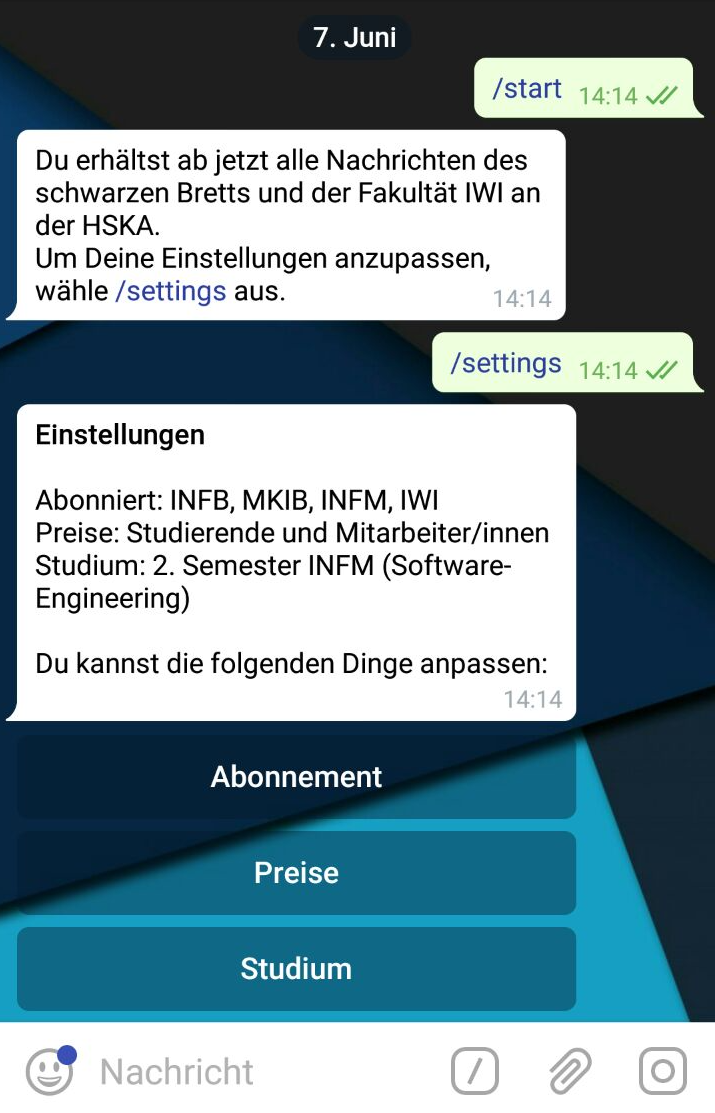
\includegraphics[width=0.4\linewidth]{settings-overview.png}
      \label{img:settings}
    \caption*{Quelle: Eigene Abbildung}
\end{figure}

Die Abonnement-Einstellung an sich hat sich zu der vorherigen Version nicht geändert, hier lässt sich der eingestellte Wert durch Inline-Buttons toggeln und eine Benachrichtung erläutert den eingestellten Wert. Die Mensapreis-Einstellung hingegen hat sich in dieser Version geändert. Hier wurde zuvor über die drei verschiedenen Werte (Studierende / Mitarbeiter / Beides) getoggelt. Dies wird in dieser Version umgangen, indem die einzelnen Optionen selektiert werden können und man mit der Selektion direkt zum Haupt-Screen zurückgelangt. Prinzipiell gibt es für alle Untermenüs die Option, zum Haupt-Screen zurückzugelangen.

\begin{figure}[H]
    \centering
    \caption{Setzen der Mensapreise}
      
\includegraphics[width=0.5\linewidth]{Mensapreise.png}
      \label{img:mensapreise}
    \caption*{Quelle: Eigene Abbildung}
\end{figure}

Die neueste Einstellung ist die Studiumseinstellung, bei der ein User sein aktuelles Semester wählen kann, um seinen Stundenplan abzufragen. Hierbei wird der User durch ein Menü geführt, bei dem er zuerst sein Studium auswählt, dann seine Vertiefungsrichtung. Dies passiert nur bei der Selektion von \texttt{INFM} passiert. Zum Schluss wählt man sein Semester. Mit Auswahl des Semesters gelangt der User zurück zu Hauptseite und die Einstellung wird übernommen. Dies wird zusätzlich durch eine Benachrichtigung kommuniziert. \\
Das besondere in diesem Fall ist die tiefere Menüführung, da man die bereits selektierten Werte zwischenspeichern muss. Dies wird über Tags gemacht, die in den Buttons gespeichert werden, somit muss der Bot den State nicht speichern, sondern dies geschieht clientseitig. Dies ermöglicht eine flexiblere Handhabung.

Der Befehl \texttt{/settings} wurde nicht nur aufgrund seines guten Namens gewählt, sondern ist ein von Telegram nativ unterstützter Befehl (siehe~\Autoref{sec:commands}). Dies fördert also zusätzlich die User-Experience.

\section{Grundfunktionalitäten}
Wie in der Einleitung bereits beschrieben, wurde auch an der Stabilität des Bots gearbeitet. Dies bezieht sich primär auf einen hartnäckigen Bug, der erst nach einiger Zeit gefunden wurde und dessen Auftreten so nicht klar war. \\
Bei dem Bug handelt es sich um eine Limitierung, die das Versenden von Nachrichten betrifft. Telegram fordert, dass nicht mehr als 30 Nachrichten pro Sekunde verschickt werden können, ansonsten wird das Versenden blockiert und  der HTTP-Fehlercode 429 zurückgegeben. Dieser Fehler ist in frühen Phasen so nicht aufgetreten, da ursprünglich nicht genug Personen von dem Bot angesprochen wurden. Außerdem wurden in einer früheren Implementierung Nachrichten einfach verschickt, ohne dass geprüft wurde, ob das Versenden überhaupt erfolgreich war. Erst beim Betrachten des Ergebnisses fiel auf, dass das Versenden nicht immer erfolgreich war. Somit wurden Maßnahmen getroffen, damit das Auftreten solcher Fehler in Zukunft vermieden werden können. \\
Momentan nutzen über 75 User den Bot, sodass das batchartige Versenden von Nachrichten zu dem Auftreten des beschriebenen Fehlers führen. Durch das getimte Versenden von Nachrichten kann dies leicht umgangen werden. Dies bedeutet, dass zwischen dem Versenden von Nachrichten 50 Millisekunden gewartet wird. Hierdurch können 20 Nachrichten pro Sekunde verschickt werden. Es sind zwar 30 Nachrichten zulässig, aber um den Latenzproblemen vorzubeugen und auch das Senden von Antworten auf Anfragen weiterhin zu gewährleisten wurde die Grenze absichtlich unterschritten. \\
Durch diese Optimierung ist zwar eine Besserung erzielt worden, aber ein sicheres Versenden wird nicht gewährleistet. Aufgrund dessen wird zusätzlich geprüft, ob das Versenden erfolgreich war und bei Auftreten des Fehlercodes 429 wird die Nachricht erneut abgeschickt. Dies wird fünf Mal versucht, danach wird die Nachricht als unzustellbar erklärt.

Intern werden \texttt{Akka-Aktoren} verwendet um die nebenläufige Abwicklung von Aufgaben zu bewerkstelligen. Diese Aktoren werden auch für das Versenden der Nachrichten eingesetzt. Es ist neben der Telegram-API-Limitierung zudem zu internen Fehlern gekommen, wenn zu viele Nachrichten auf einmal geschickt wurden, da der interne Threadpool überlief. Auch dieses Problem wird durch das verzögerte Senden behoben. \\
Außerdem wurden einige Teile des Programms refaktoriert, damit der Code lesbarer und sicherer läuft.

\section{Caching}
Da besonders die Anfrage nach den Vorlesungsinformationen große Datenmengen laden und verarbeiten muss und die Informationen sich im Allgemeinen nicht häufig ändern, werden diese gecacht. Ursprünglich sollte dieses Caching manuell erfolgen, indem die Resultate der HTTP-Anfragen in der Redis-Datenbank gespeichert werden. Dies ist jedoch nicht sinnvoll, da besonders Verfahren wie das Invalidieren des Caches nicht unbedingt trivial sind und es sich bewährt hat, etablierte Frameworks und Bibliotheken eigenen Lösungen zu bevorzugen.

In der Java-Welt ist eine der größten Caching-Bibliotheken \texttt{Caffeine}\footnote{\url{https://github.com/ben-manes/caffeine}}. Diese Bibliothek bietet einen einfachen Key-Value-Store, der getypte Elemente beinhalten kann. So müssen Daten nicht unbedingt serialisiert abgelegt werden, sondern können als Datenobjekt dort gecacht und direkt abgerufen werden. Das Ziel von Caffeine ist eine hohe Performance und es wird eine sehr intuitive API angeboten. Um den Einsatz mit Scala etwas zu erleichtern gibt es einen Scala-Layer, der die Caffeine-API abstrahiert und an Scala-Syntax anpasst.~\footnote{\url{https://github.com/blemale/scaffeine}}

Der Cache liegt direkt im Hauptspeicher und man kann für den gesamten Cache eine Invalidierungszeit angeben, also die Zeit, die Elemente im Cache liegen sollen bis sie invalidiert werden.\\
Der Cache des IWINews Bots wird direkt in der Klasse, die für die HTTP-Aufrufe zuständig ist, angelegt, um das Caching vor den Aufrufen zu verstecken. In dem Cache wird als Schlüssel die URL gewählt, der Wert ist das Ergebnis der Anfrage, da der Cache generisch gehalten werden muss. Wird eine HTTP-Anfrage verlangt, wird geprüft, ob ein Wert im Cache für die angefragt URL liegt, wenn dies der Fall ist, wird der Wert aus dem Cache geholt. Ist noch kein Wert im Cache, wird die URL aufgerufen, die Antwort wird im Cache gespeichert und zurück gegeben.

Da die Anfragen, ob es neue Nachrichten auf dem schwarzen Brett gibt, jedoch nicht gecacht werden soll, da so Änderungen nicht entdeckt und somit auch nicht verbreitet werden können, ist es notwendig eine spezielle Methode einzuführen, die einen HTTP-Aufruf ohne Cache macht. Dieser Aufruf entspricht dem bisherigen Verfahren und konnte somit einfach übernommen werden, auch wenn dieser Aufruf umbenannt werden musste um sicher zu gehen, dass dies ein Sonderfall ist. Wie das Caching konkret umgesetzt ist, wird in \autoref{caching} gezeigt.

\lstinputlisting[language=scala, style=scala, numbers=none, caption={Erweiterung der HTTP-Anfragen um Caching-Mechanismus}, label=caching, firstline=5, lastline=52]{HTTPGet.scala}

\chapter{Proof-of-Concept: Sprachnachrichten}
Neben der klassischen Chatbot-Funktion, bei der ein User per Textnachrichten mit dem Bot redet, ist es vor allem in letzter Zeit immer mehr zum Usus geworden, dass man mit Bots reden möchte, um Informationen zu erhalten.  \\Produkte wie Google Home und Amazons Alexa sind hierfür die bekanntesten Vertreter, die eine solche Funktion bieten. Während des Brainstormings zu Use-Cases des Chatbots kam zudem die Idee auf, dass der Chatbot nicht nur auf Chat-Nachrichten antworten, sondern auch auf Sprachnachrichten reagieren können sollte. \\
Hier bietet Telegram die Möglichkeit, kurze Sprachnachrichten direkt zu versenden. Wenn der Bot diese Sprachnachricht zu Text übersetzen könnte, ist es möglich, diesen verstandenen Text durch den Chatbot zu verarbeiten und entsprechend zu antworten. \\
Da der produktive Einsatz eines solchen Features nicht wahrscheinlich ist, sollte es als Proof-of-Concept untersucht und exemplarisch implementiert werden.

\section{Architekturentwurf}
Telegram bietet mit seinen Sprachnachrichten bereits die Möglichkeit, Sprache aufzunehmen und zu versenden. Diese Sprachnachrichten können nicht nur zwischen zwei Personen verschickt werden, sondern auch zwischen einer Person und einem Bot versandt werden. Telegram unterstützt die mobilen Betriebssysteme \texttt{iOS} und \texttt{Android}. Am Desktop lässt es sich über \texttt{MacOS}, \texttt{Windows}, \texttt{Linux} und im Webbrowser bedienen. Durch eine direkte Integration in diese Telegram-Clients, ist es also sehr einfach, solche Nachrichten zu versenden.

\subsection{Speech-to-Text}
Die Interpretation der Sprachnachricht erfolgt durch Rivescript, was Texteingaben verarbeitet und Textausgaben erzeugt. Somit ist es notwendig, dass die Spracheingabe zu Text verarbeitet wird, was im Allgemeinen als Speech-to-Text bezeichnet wird. Diese Umwandlung ist nicht trivial und wird mittels Machine-Learning möglich gemacht. Anstatt die Umwandlung selber zu machen, wurde sie in diesem Projekt exemplarische Googles-Cloud-Services erzeugt. Google setzt auf Machine-Learning und hat durch seine große Nutzerzahl und vielseitige Nutzung gut trainierte Modelle, sodass die Sprache zuverlässig verstanden werden kann.

\subsection{Google-Cloud-Speech-API}
Die Google-Cloud-Speech-to-Text-API ist ein SAAS-Angebot, bei dem man Sprachdateien an den Google-Server senden kann und diese Sprachdateien von dem Service interpretiert und zu Text umgewandelt werden, den man als einfaches JSON-Objekt erhält. Da die Umwandlung von Sprache zu Text auf der Wahrscheinlichkeit beruht, dass etwas korrekt verstanden wurde, wird diese Genauigkeit mitzurückgegeben. Sollte die Eingabesprache nicht eindeutig sein, so werden mehrere Ergebnisse mit der jeweiligen Genauigkeit zurückgegeben.
Der Cloud-Service wird über HTTP angesprochen, man muss jedoch eine Authentifizierungstoken einreichen. Hierfür muss man sich einen Google-Developer-Account erstellen und muss die API aktivieren. Der Service kostet für gewöhnlich Geld, hierbei werden 0,006\$/15 Sekunden berechnet.~\footnote{\url{https://cloud.google.com/speech-to-text/}} \\
Man kann den Service jedoch kostenlos nutzen, wenn man pro Tag weniger als 60 Minuten an Eingabe verarbeitet. Zusätzlich erhält man bei der Eröffnung eines Accounts ein Guthaben in Höhe von 300\$, sodass man die Services ausgiebig testen kann.

Das folgende Schaubild soll einen exemplarischen Ablauf erklären:
\begin{figure}[H]
    \centering
    \caption{Kommunikationsprozess}
      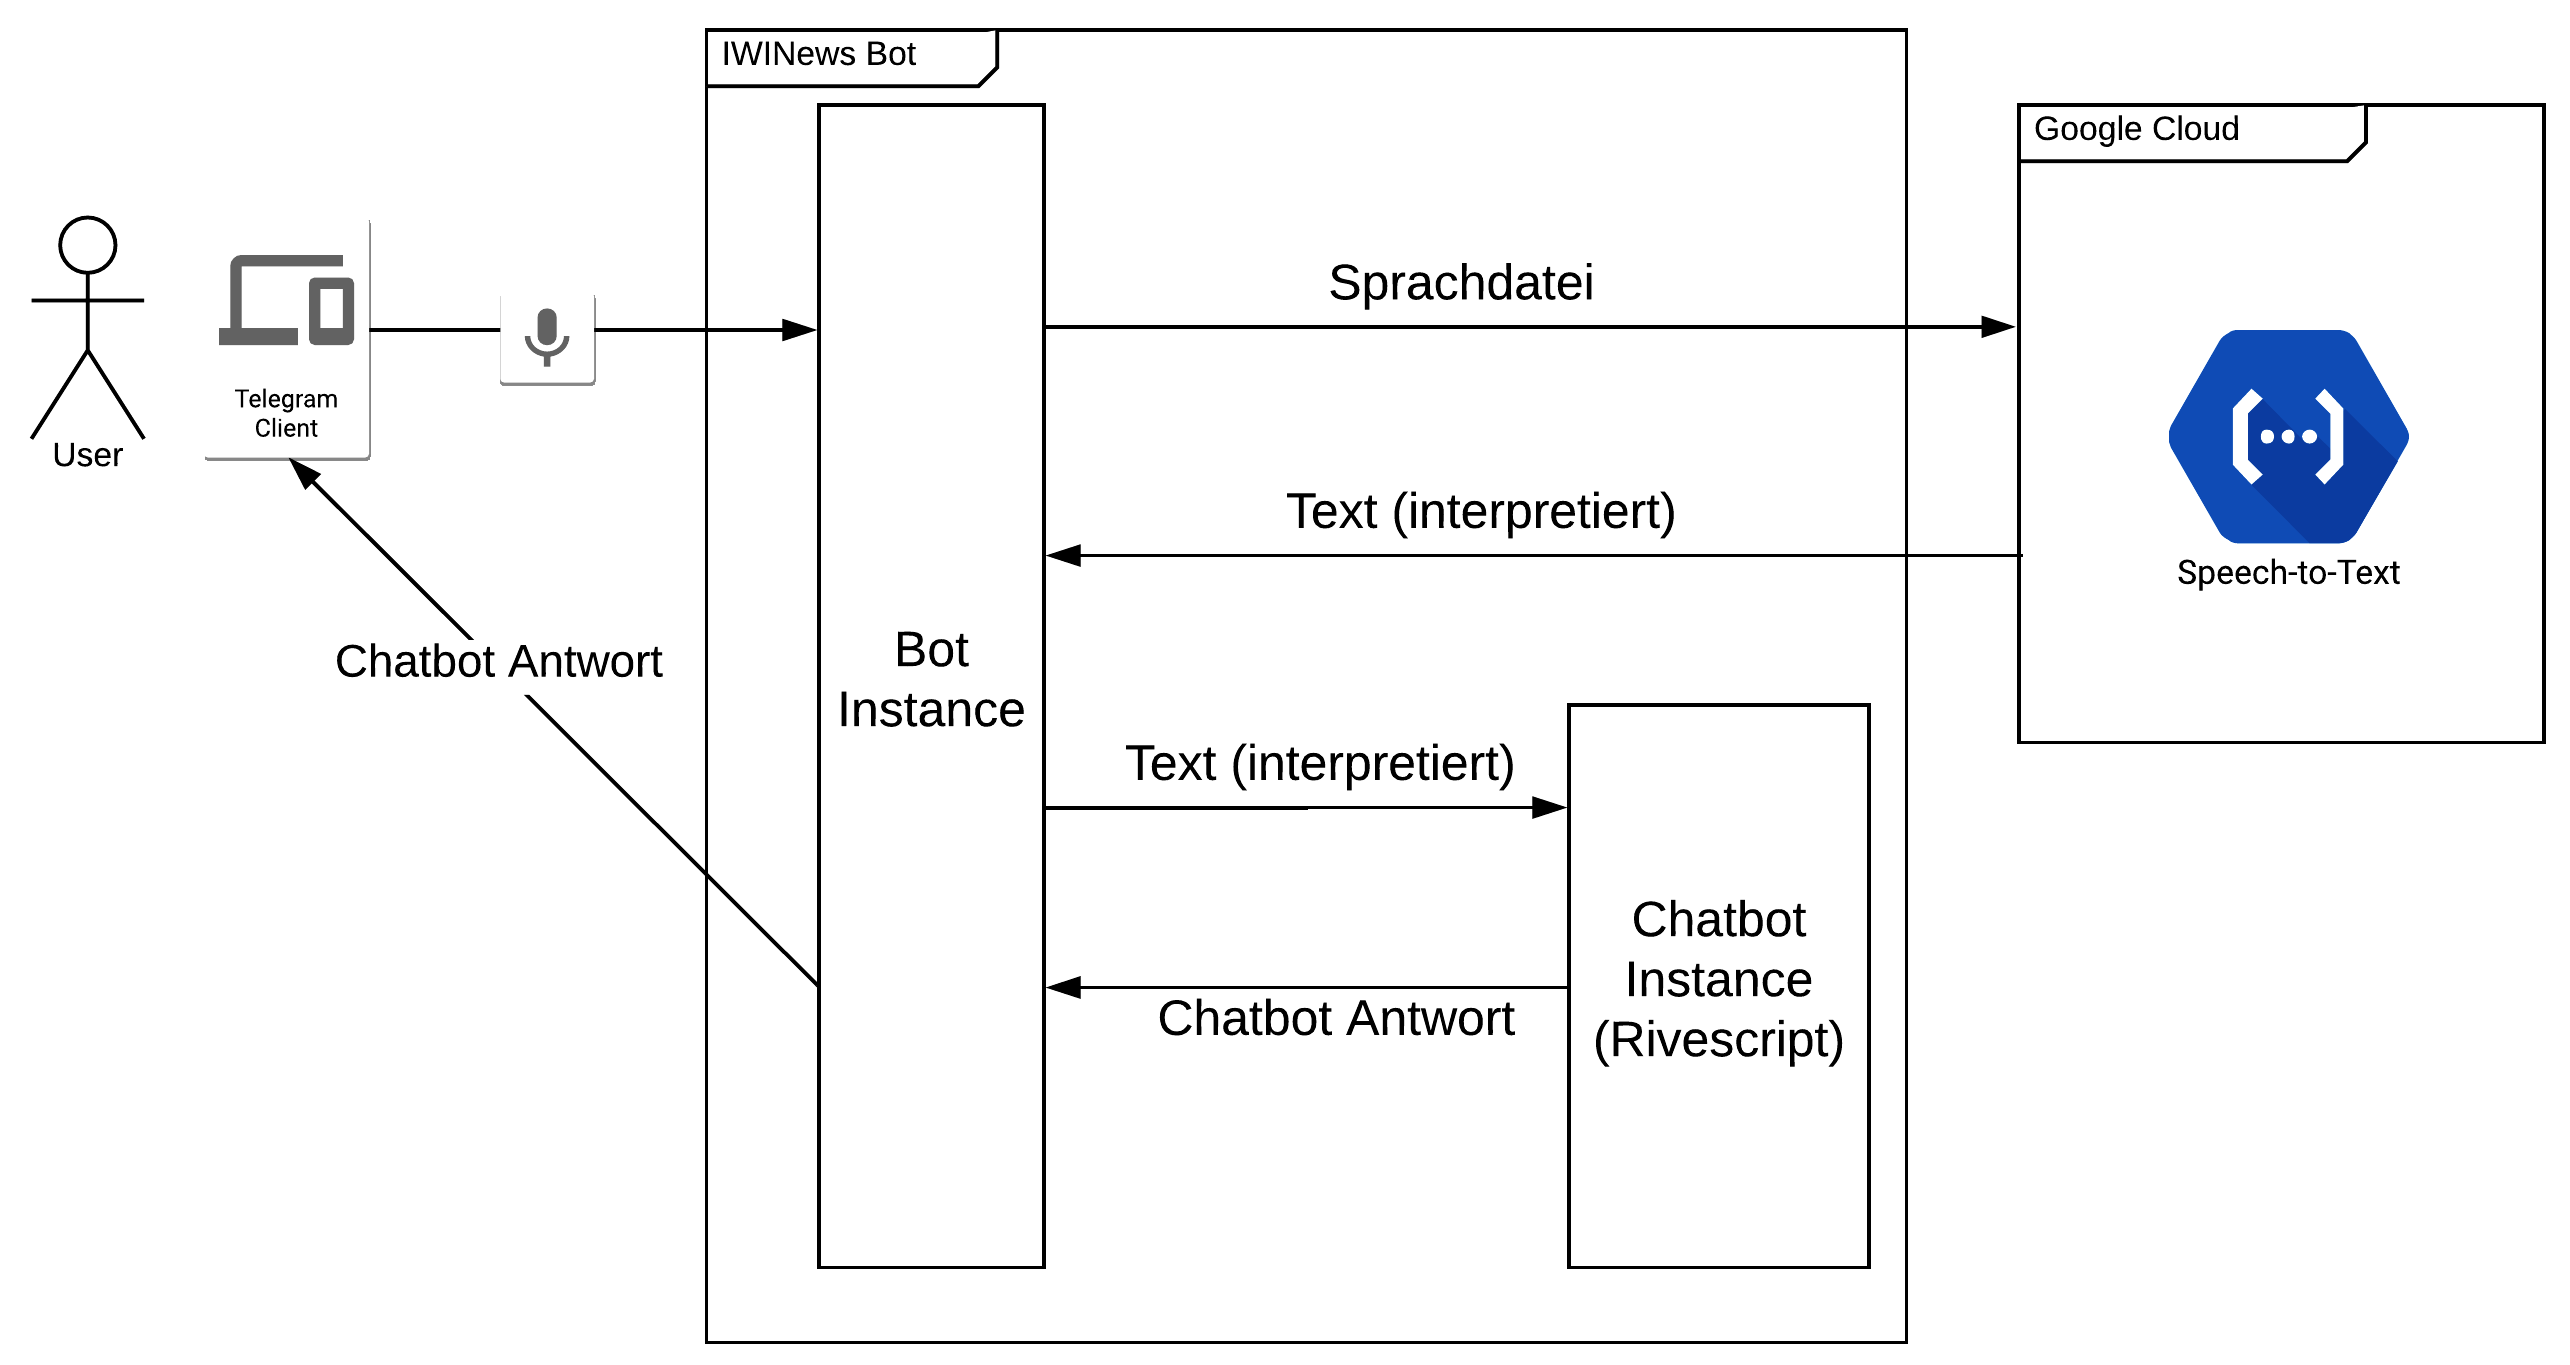
\includegraphics[width=\linewidth]{ArchitekturTelegramBot.png}
      \label{img:architektur}
    \caption*{Quelle: Eigene Abbildung}
\end{figure}

\subsubsection{Java-Bibliothek}
Google bietet eine Java-Bibliothek an, um den Aufruf der API zu abstrahieren und somit zu vereinfachen. Hierbei wird sowohl die Authentifizierung, als auch die Anfrage mit den einzelnen Parametern stark vereinfacht. Diese Bibliothek befindet sich jedoch noch im Alpha-Modus und sollte somit auf keinen Fall in produktiven Umgebungen eingesetzt werden. Auch in diesem Projekt sind Warnungen beim Bauen mit \texttt{sbt} aufgetreten und es wurde ein Issue auf Github eröffnet, sodass dieses Problem für das Release gefixt wird.~\footnote{\url{https://github.com/GoogleCloudPlatform/google-cloud-java/issues/3329}} 
Die Einbindung der Bibliothek ist jedoch sehr einfach, da sie auf Maven-Central gehostet wird.

\subsubsection{Authentifizierung}
Das Token, das zur Authentifizierung genutzt wird, ist in einer \texttt{.json}-Datei gespeichert, die man in der Google-Developer-Console downloaden kann. Diese \texttt{.json}-Datei muss dem Programm, das die Google-API ansprechen möchte, bekannt gemacht werden, was am einfachsten über die Pfadvariable \texttt{GOOGLE\_APPLICATION\_CREDENTIALS} gemacht wird. Diese Pfadvariable wird dann von der Bibliothek gelesen und zur Authentifizierung genutzt. Da in der Pfadvariable nicht der Inhalt der \texttt{.json}-Datei, sondern der Pfad zur \texttt{.json}-Datei gespeichert wird, darf man diese Datei nicht löschen oder verschieben.

\section{Implementierung}
Nachdem nun die relevanten Technologien und deren Zusammenspiel beschrieben wurden, soll vorgestellt werden, wie die Interpretation der Sprachnachrichten konkret funktioniert und wie es umgesetzt wurde.

\subsubsection{Beispiel}
Bevor auf die Implementierungsdetails eingegangen wird, soll die Funktionsweise vorgestellt und erläutert werden.

\begin{figure}[!htb]
    \centering
    \caption{Beispiel der Verwendung von Speech-to-Text}
      
\includegraphics[width=0.5\linewidth]{Sprachnachrichten_Beispiel.png}
      \label{img:speekExample}
    \caption*{Quelle: Eigene Abbildung}
\end{figure}

Wie man an dem Beispiel bereits erkennt, gibt es eine Quota, die speichert, wie viel von dem Kontingent für Sprachnachrichten bereits verbraucht wurde. Außerdem werden zu lange Nachrichten, also Nachrichten die Länger als sieben Sekunden dauern, abgewiesen. Durch diese Mechanismen wird vermieden, dass die Sprachnachrichten missbraucht werden und die Ressourcen des Google-Cloud-Service zu sehr beansprucht werden.
Neben den Einschränkungen erkennt man aber an dem Beispiel zusätzlich, dass die Sprachnachricht von dem Bot korrekt erkannt wird und anschließend vom Chatbot beantwortet wird.

\subsection{Empfangen von Sprachnachrichten}
So wie bereits für die Chat-Nachrichten, muss der Bot so erweitert werden, dass er Sprachnachrichten empfangen kann. Dies geschieht über das Reagieren auf eingehende Nachrichten und das Überprüfen, ob es sich um eine Sprachnachricht handelt. Ist dies der Fall, so können bereits Eigenschaften der Sprachnachricht abgefragt werden, beispielsweise die Dauer. Dies ist sinnvoll, da über die Dauer entschieden wird, ob die Nachricht verarbeitet wird, oder nicht.

\lstinputlisting[language=scala, style=scala, caption={Empfangen von Sprachnachrichten}, label=speech1, firstline=1, lastline=13]{ChatSpeech.scala}

Wie man in~\Autoref{line:quotaRedis} bereits erkennt, wird die Quota in der Redis-Datenbank gespeichert, sodass diese persistiert wird. Der User wird in dem Fall, dass die Quota für den Tag überschritten wird, mit einer Fehlermeldung über den Umstand informiert, zusätzlich wird der Vorfall geloggt. \\
Sollte die Quota noch nicht erschöpft sein und die Sprachnachricht ist kurz genug, wird die Datei geladen. Telegram sieht hierbei vor, dass ein Link generiert werden muss, über den die Sprachdatei dann geladen werden kann. Der Link folgt der folgenden Struktur:

\url{https://api.telegram.org/file/botBottoken/Filetoken}

Das \texttt{Bottoken} ist dabei das Token, das zu Identifizierung des Telegram-Bots genutzt wird und in der Datei \texttt{bot.token} gespeichert ist. Das \texttt{Filetoken} muss erst generiert werden. Für die Generierung dieses Filetokens bietet das \texttt{Telegrambot4s}-Framework einen eigenen \texttt{request}-Aufruf an, der dieses Token als \texttt{filePath} zurückgibt. Dies geschieht wie folgt:

\lstinputlisting[language=scala, style=scala, caption=Generierung des Filetokens, label=filetoken, firstline=15, lastline=22]{ChatSpeech.scala}

Über die URL kann dann die Sprachdatei heruntergeladen werden. Diese wird lokal in dem Ordner \texttt{voices/} abgelegt, dabei wird das Datum und die Uhrzeit, sowie die \texttt{userID} im Dateinamen gespeichert.
Diese Datei wird benötigt, um die darin enthaltene Sprache in Text umzuwandeln. Hier kommt also der Google-Cloud-Service ins Spiel.

\subsection{Konfiguration des Speech-Client}
Die Google-Cloud-API bietet eine Klasse des Typs \texttt{SpeechClient} an, über die die einzelnen Anfragen an den Google-Cloud-Service gestellt werden. Dieser muss entsprechend konfiguriert sein, damit die in den Sprachdateien enthaltene Sprache auch korrekt verstanden und zu Text transkribiert werden kann. \\
Die Sprachdateien liegen im \texttt{OGG}-Dateiformat vor. Ein Großes Problem bei der Entwicklung war dabei die Frequenz, da diese dem SpeechClient mitgeteilt werden muss. Hier wurde davon ausgegangen, dass alle Telegram-Clients auf das selbe Dateiformat mit derselben Frequenz setzen, was aber nicht der Fall ist. Gibt man die falsche Frequenz einer Sprachdatei an, kann Google den Inhalt nicht verstehen und gibt ein leeres Ergebnis zurück. Der Fehler fiel beim Testen mit verschiedenen Geräten auf und die Behebung erfolgte durch reines Herumprobieren bei den Frequenzen. \\
Nachdem das Problem lokalisiert wurde, war die Lösung verhältnismäßig einfach. Die Frequenz der lokalen Datei wird aus der Datei gelesen und dem SpeechClient mitgeteilt. Hierzu wird eine zusätzliche Bibliothek benötigt, die diese Funktion bereitstellt. Außerdem muss dem SpeechClient mitgeteilt werden, um welche Sprache es sich bei der Eingabe handelt, diese Erkennung erfolgt nicht automatisch. Die vollständige Konfiguration wird im Folgenden gezeigt.

\lstinputlisting[language=scala, style=scala, caption=Erstellen des Requests zur Spracherkennung, label=request, firstline=24, lastline=32]{ChatSpeech.scala}

Da die Bibliothek für Java-Programme geschrieben wurde, gilt es, das Ergebnis in eine Scala-Collection umzuwandeln, um die Ergebnisliste einfacher traversieren zu können.

Das erste Ergebnis ist für gewöhnlich das beste Ergebnis, dies wird an die Rivescript-Instanz übergeben und dort weiter verarbeitet. Dies geschieht wie bereits mit den Textnachrichten. \\
Kann eine Sprachnachricht nicht verstanden werden, etwa weil die Umgebungsgeräusche zu laut sind oder der Sprecher zu undeutlich spricht, wird entsprechend eine Fehlermeldung ausgegeben. \\
Bei jeder Anfrage an den Google-Cloud-Service wird die Dauer der Sprachnachricht der Quota hinzugefügt.

\chapter{Fazit}
Am Ende dieser Arbeit wird aus den gewonnenen Erfahrung mit der Telegram-Bot-API ein Resumee gezogen. Zuletzt werden Anstöße zur weiteren Entwicklung des Hochschul-Bots gegeben.

\section{Bewertung}
\section{Ausblick}

\newpage
\phantomsection\addcontentsline{toc}{chapter}{Abbildungsverzeichnis}
\listoffigures
\clearpage

\phantomsection\addcontentsline{toc}{chapter}{Quellcodeverzeichnis}
\lstlistoflistings\clearpage

\end{document}
